\documentclass[fontset=none,11pt,a4paper]{ctexart}
\setCJKmainfont{AR PL SungtiL GB}[BoldFont=AR PL UMing CN,AutoFakeBold=2.5]
\setCJKsansfont{AR PL UMing CN}
\setCJKmonofont{AR PL UMing CN}
\usepackage{geometry,booktabs,multirow,hyperref,enumitem,xcolor,longtable,listings,graphicx}
\geometry{margin=2.2cm}
\definecolor{codebg}{rgb}{0.95,0.95,0.95}
\lstset{basicstyle=\ttfamily\small,backgroundcolor=\color{codebg},frame=single,breaklines=true}
\title{多模态Agent Post-Training 项目\\从零到一的完整指南}
\author{}
\date{\today}

\begin{document}
\maketitle

\begin{abstract}
本文档以初学者友好的方式，完整记录多模态Agent Post-Training项目从零搭建到当前状态的每一个决策、每一次失败、每一处优化。项目目标：训练Qwen2.5-VL视觉语言模型在收到"图片+问题"后，自动按vision\_parse $\to$ retrieve\_docs/python\_exec $\to$ final\_answer的多步工具调用链完成任务。全文按数据工程、模型训练、推理评测、Agent优化四条主线展开，结合每一份代码文件解读其设计动机、解决的问题、实际效果，以及失败尝试背后的深层原因。
\end{abstract}

\tableofcontents

\section{项目概述：我们要做什么}

\subsection{一句话定义}

给模型一张发票照片和问题"这张发票缺少必填字段吗？"，模型应该自己知道：(1) 先调OCR看清发票上的字，(2) 查规则文档找必填字段清单，(3) 对比后给出有依据的结论。

这不是简单的"看图回答问题"---模型需要自己\textbf{决策每一步该调哪个工具}，而且每轮只能做一件事。

\subsection{核心约束为什么这么严格}

每轮模型只能输出一个 \texttt{<tool\_call>} 或一个 \texttt{<final\_answer>}。这个约束不是我们故意为难模型---它是"工具调用"的本质：一次只能做一个动作，做了之后等结果，根据结果决定下一步。

这个约束是整个项目最重要的设计决策，也是后来几乎所有优化失败的根源。因为大部分LLM优化方法（DPO、RL、数据增强）都假设模型输出是"一段自由文本"，而我们要求的是"严格格式的单一步骤"。

\subsection{项目代码结构总览}

项目根目录在 \texttt{/root/miniconda3/bin/multimodal-agent-posttraining(服务器)/}，有六个子目录：

\begin{itemize}[nosep]
    \item \texttt{agent/} --- 推理核心：6个py文件，负责模型的加载、推理、工具执行、输出解析
    \item \texttt{train/} --- 训练引擎：SFT LoRA训练、DPO偏好训练、自研RL训练
    \item \texttt{eval/} --- 评测系统：50条评测样本的自动评测和指标计算
    \item \texttt{scripts/} --- 数据构建管线：25个py脚本，负责数据的生成、转换、增强、分析
    \item \texttt{data/} --- 数据存储：SFT训练数据、DPO偏好数据、评测数据、规则文档、图片资源
    \item \texttt{paper/} --- 项目文档：LaTeX论文和报告
\end{itemize}

外部存储（不在项目目录内）：
\begin{itemize}[nosep]
    \item \texttt{/root/autodl-tmp/models/} --- 基座模型：Qwen2.5-VL-3B-Instruct(7.1GB) + 7B(16GB)
    \item \texttt{/root/autodl-tmp/multimodal-agent-lora/} --- 训练好的LoRA权重
    \item \texttt{/root/autodl-tmp/multimodal-agent-data/} --- 外部数据集图片(ChartQA/DocVQA/CORD，已resize)
\end{itemize}

\newpage

\section{损失函数设计：从SFT到RL的完整演化}

这一节专门讲"模型怎么知道自己学得好不好"---即每个训练阶段的损失函数（loss function）。损失函数是整个项目的灵魂：它定义了"什么是好行为"。后面的所有优化失败，归根结底都是损失函数和任务不匹配。

\subsection{SFT损失：模仿正确答案}

SFT（Supervised Fine-Tuning）的损失是最简单的交叉熵（Cross-Entropy）：

\[
\mathcal{L}_{SFT} = -\frac{1}{N}\sum_{i=1}^{N} \log P(y_i \mid x, y_{<i})
\]

\textbf{白话解释}：对于训练数据中的每个token，计算模型预测"正确token"的概率，取负对数。概率越高，loss越低。模型的目标就是不断提高"正确答案"的概率。

\textbf{代码实现}（train\_sft\_lora.py 的 QwenVLSFTCollator）：
\begin{lstlisting}
# 只有assistant输出的token才参与loss计算
# prefix（用户消息、工具结果、之前的assistant输出）被mask掉
labels[row_index, :prefix_len] = -100  # -100 = 不计算loss
\end{lstlisting}

\textbf{为什么prefix要mask}：我们只希望模型学会"在这个上下文中应该输出什么"，而不是让它"重新学习"所有的上下文。如果prefix也算loss，模型会浪费大量计算在复制已有的对话史上。

\textbf{SFT的优点}：简单、稳定、收敛快。
\textbf{SFT的缺点}：模型只能模仿训练数据中的行为，不能超越。如果数据中"直接回答"和"调工具后回答"的比例出了问题，模型就学歪了。

\subsection{DPO损失：偏好比较（已弃用）}

DPO的目标不是"模仿正确答案"，而是"A比B好"：

\[
\mathcal{L}_{DPO} = -\log\sigma\left(\beta \cdot (\log\frac{\pi_\theta(y_{chosen}|x)}{\pi_{ref}(y_{chosen}|x)} - \log\frac{\pi_\theta(y_{rejected}|x)}{\pi_{ref}(y_{rejected}|x)})\right)
\]

\textbf{白话解释}：chosen（好答案）和 rejected（坏答案）各算一个"得分"---模型对它的log-prob除以参考模型对它的log-prob。如果chosen的得分明显高于rejected，loss就低。$\beta$（通常0.1）控制偏好强度，$\sigma$是sigmoid函数（把任意值压到0-1之间）。

\textbf{在这个项目里为什么失败}：

关键问题：$\pi_\theta(y|x)$ 中的 $y$ 是什么？

在标准DPO中，$y$是\textbf{完整的回答}。但我们的任务是多轮的---每次对话包含3-5轮交替的assistant输出和tool结果。DPO的代码实现（compute\_log\_prob）只取了\textbf{最后一条}assistant消息：

\begin{lstlisting}
# train_dpo_lora.py: 只计算最后一条assistant消息的log-prob
assistant_idx = last_assistant_message(messages)
prefix = messages[:assistant_idx]  # 前面的全部内容
full = messages[:assistant_idx + 1]  # 包含最后的assistant

# 只优化 P(最后的assistant | 前面的全部上下文)
\end{lstlisting}

这导致DPO\textbf{只优化最终答案}，不优化工具调用步骤。当偏好数据是单轮的时候（user $\to$ final\_answer），模型学到的就是"直接从问题跳到答案"---和SFT教的"先调工具再回答"直接冲突。

\textbf{因此}：DPO在标准对话任务中有效，但在多轮工具调用任务中与SFT的格式纪律产生根本性冲突。

\subsection{RL Reward函数：多维度打分}

REINFORCE/GRPO不用固定的"正确答案"，而是用reward函数\textbf{实时打分}。模型自己生成rollout，然后reward函数评判"这次做得好不好"。

\textbf{当前reward函数}（train\_rl\_custom.py 的 compute\_reward）：

\begin{lstlisting}
def compute_reward(result, gold):
    reward = 0.0
    # 1. 格式正确性（最高权重，-2表示绝不容忍格式错误）
    if result.status == "parse_error":   reward -= 2.0
    # 2. 工具选择（+1正确调用，-0.5漏调，+0.5正确不调）
    if needs_tools and tools_correct:    reward += 1.0
    elif needs_tools and tools_wrong:    reward -= 0.5
    elif no_tools_needed and no_tools:   reward += 0.5
    # 3. 答案质量（+0.5包含关键词/数值）
    if keywords_in_answer:               reward += 0.5
    # 4. 拒答正确性（+0.5该拒答时拒了）
    if refusal_correct:                  reward += 0.5
    # 5. 冗余工具惩罚（-0.3该不调时调了）
    if no_tools_needed and tools_called: reward -= 0.3
    return reward  # 范围约 [-2.8, +2.5]
\end{lstlisting}

\textbf{权重设计逻辑}：
\begin{itemize}[nosep]
    \item \textbf{格式罚分最重(-2.0)}---因为没有格式就没有一切。格式错了后面的工具调用和答案都没意义
    \item \textbf{工具选择权重最高(+1.0)}---这是Agent最核心的能力
    \item \textbf{正确答案和拒答各+0.5}---次优先级，内容好但格式对至少还能用
    \item \textbf{冗余工具轻罚(-0.3)}---多调一个工具比漏调好，保守策略
\end{itemize}

\subsection{REINFORCE损失：奖励引导的梯度}

REINFORCE是最基础的RL算法。它的核心思想和SFT完全相反：

\begin{itemize}[nosep]
    \item SFT：告诉模型"正确答案是什么"，照着学
    \item REINFORCE：让模型自己试，试完根据分数决定"往哪个方向改"
\end{itemize}

\[
\mathcal{L}_{REINFORCE} = -\frac{1}{K}\sum_{i=1}^{K} A_i \cdot \frac{1}{T_i}\sum_{t=1}^{T_i} \log\pi_\theta(token_t \mid context)
\]

\textbf{白话解释}：
\begin{enumerate}[nosep]
    \item 同一个问题让模型试K=4次（4次rollout），每次得到不同的trace
    \item 每次rollout根据reward函数打分，得到4个分数 $r_1, r_2, r_3, r_4$
    \item 计算\textbf{优势}（advantage）：$A_i = \frac{r_i - mean(r)}{\text{std}(r)}$---这次rollout比平均水平好多少
    \item 如果某次rollout的advantage为正（比平均好），就\textbf{增大}这次rollout中每个决策token的概率
    \item 如果advantage为负（比平均差），就\textbf{减小}概率
    \item 梯度方向 = $-A_i \times \nabla\log\pi_\theta$---advantage是梯度的"缩放因子"
\end{enumerate}

\textbf{代码实现}：
\begin{lstlisting}
# train_rl_custom.py 的 REINFORCE loss
plp = compute_turn_log_prob(policy_model, messages, turn_idx)  # log P(token|context)
reinforce = -advantage * plp.mean()  # 负号: 最大化优势为正的行为
\end{lstlisting}

\subsection{KL惩罚：安全绳}

REINFORCE有一个风险：模型为了最大化reward，可能会"走火入魔"---比如发现"输出空字符串能避免parse\_error罚分"，于是完全不输出内容。

\textbf{KL惩罚}（Kullback-Leibler Divergence Penalty）就是解决这个问题的：

\[
\mathcal{L}_{KL} = \beta \cdot \frac{1}{T}\sum_{t=1}^{T} (\log\pi_\theta(token_t) - \log\pi_{ref}(token_t))
\]

\textbf{白话解释}：如果当前策略($\pi_\theta$)和参考策略($\pi_{ref}$, 即SFT模型)对同一个token的log-prob差太多，就加惩罚。$\beta$=0.2控制惩罚强度---太大则模型不敢动（和SFT一样），太小则可能跑飞。

\textbf{为什么用SFT做参考而不是上一轮策略}：SFT是"已知安全的"，用SFT做锚点保证模型不会偏离到格式崩溃的区间。$\pi_{old}$（上一轮策略）虽然更标准，但在这个项目中，SFT的格式纪律已经过验证，用它做锚更稳定。

\subsection{完整RL损失}

最终的RL损失是REINFORCE和KL的加权和：

\[
\mathcal{L}_{total} = -\frac{1}{K}\sum_{i=1}^{K} A_i \cdot \log\pi_\theta(y_i) \;+\; \beta \cdot \frac{1}{T}\sum_{t=1}^{T} (\log\pi_\theta(y_t) - \log\pi_{ref}(y_t))
\]

\textbf{为什么ratio=1（不用重要性采样）}：

标准GRPO会在REINFORCE外乘以ratio($\pi_\theta/\pi_{old}$)，这是"重要性采样校正"---因为本次rollout是用$\pi_{old}$生成的，但我们要优化$\pi_\theta$，需要校正。

在我们的实现中，ratio始终=1（即不做校正）。原因是：
\begin{enumerate}[nosep]
    \item Agent的每次rollout产生\textbf{不同的}多轮文本，无法跨轮比较
    \item 缓存按位置匹配（同一个(id, rollout\_idx, turn\_idx)），但文本内容每轮都变
    \item ratio比较的是两个不同文本的概率，无意义
    \item 纯REINFORCE虽然方差大，但至少是正确的
\end{enumerate}

\textbf{3B reward不动的原因}：V4的4次rollout得分几乎一样（tools都100\%正确，答案质量相近），组内advantage $\approx$ 0，梯度信号为零。

\textbf{7B有空间的原因}：V7B-clean的工具命中只有92\%，存在"正确调工具"和"跳过工具"的真实分化，advantage有区分度。

\section{概念速查：10分钟理解所有术语}

如果你是完全的新手，先读这一节。每个概念用一句话+一个比喻解释。

\begin{longtable}{lp{9cm}}
\toprule
术语 & 一句话解释 \\
\midrule
\textbf{VLM} & Visual Language Model，视觉语言模型。能同时"看"图片和"读"文字的AI。 \\
\textbf{Qwen2.5-VL} & 阿里开源的一个VLM系列，有3B和7B两个规模。B=Billion(十亿参数)。 \\
\textbf{3B vs 7B} & 参数越多，模型越"聪明"（视觉理解更好），但也越"敏感"（容易走捷径）。 \\
\textbf{LoRA} & Low-Rank Adaptation。不修改原模型，只训练一个很小的"补丁"挂上去。省显存，也方便切换。 \\
\textbf{SFT} & Supervised Fine-Tuning。给模型看"正确答案"，让它模仿。像老师教学生抄正确答案。 \\
\textbf{DPO} & Direct Preference Optimization。不给正确答案，只告诉模型"A比B好"。像品酒师告诉你哪杯更好。 \\
\textbf{GRPO} & Group Relative Policy Optimization。让模型自己试K次，挑最好的，下次往那个方向走。像投篮---投4次，进了的记住手感。 \\
\textbf{RL/REINFORCE} & Reinforcement Learning。模型自己探索，好行为加分，坏行为扣分。像训练狗---做对了给零食。 \\
\textbf{KL惩罚} & Kullback-Leibler divergence penalty。防止模型在RL训练中"跑太远"忘记原本的能力。像安全绳。 \\
\textbf{tool\_call/final\_answer} & 模型的两种输出。前者是"我要调工具"，后者是"我要给答案了"。每轮只能选一个。 \\
\textbf{enforce} & Runtime拦截。如果模型想偷懒直接给答案，runtime检查"你是不是漏了某个工具？"，漏了就拦回去。 \\
\textbf{rollout} & 一次完整的Agent运行。从用户提问到最终答案的整个过程，包含多轮工具调用。 \\
\textbf{reward} & 奖励分数。一次rollout结束后，根据工具是否正确、答案是否准确、格式是否规范打分。 \\
\textbf{advantage} & 相对优势。同一样本的K次rollout中，这次rollout比平均水平好多少。归零中心化后的reward。 \\
\textbf{log-prob} & 对数概率。模型对自己输出的每个token的"自信程度"。RL用它乘以advantage决定梯度方向。 \\
\bottomrule
\end{longtable}

\section{推理系统：agent/ 目录详解}

推理系统是整个项目的"执行层"---训练好的模型在这里真正运行。理解推理系统是理解训练数据格式和评测逻辑的基础。

\subsection{agent/vlm.py --- 模型的加载和推理}

\textbf{动机}：Qwen2.5-VL是一个视觉语言模型，加载它需要同时处理文本和图片输入。此外，我们训练好的LoRA adapter需要"挂载"到基座模型上。这些操作比较复杂，封装成一个类可以复用。

\textbf{核心类 QwenVLModel}：

\begin{lstlisting}
class QwenVLModel:
    def __init__(self, model_name, adapter_name=None, max_new_tokens=512, use_mock=None):
        # 1. 检查依赖是否可用（transformers, peft, qwen_vl_utils）
        # 2. 如果依赖缺失或明确要求，进入mock模式
        # 3. 否则加载真实模型 + 可选的LoRA adapter
\end{lstlisting}

\textbf{设计要点}：
\begin{itemize}[nosep]
    \item \textbf{mock模式}：当真实VLM依赖不可用时，用一个简单的规则引擎代替。它根据用户问题中的关键词（"发票""图表""品牌"）和图片文件名来猜测应该输出什么。这让我们在没有GPU的环境下也能跑通代码流程。
    \item \textbf{LoRA注入}：如果传入了adapter\_name，通过PeftModel.from\_pretrained加载LoRA权重。这是"即插即用"的设计---同一个基座模型可以挂不同的adapter切换能力。
\end{itemize}

\textbf{generate方法}：
\begin{lstlisting}
def generate(self, messages):
    if self.use_mock:
        return self._mock_generate(messages)  # 规则引擎
    # 真实推理：apply_chat_template -> process_vision_info -> model.generate -> decode
\end{lstlisting}

\textbf{协作关系}：被 runtime.py（Agent推理）和 eval/run\_vlm\_eval.py（评测）使用。train/train\_rl\_custom.py 中通过 PolicyModelWrapper 包装它。

\subsection{agent/parser.py --- 解析模型输出}

\textbf{动机}：模型输出是自由文本，但Agent需要知道"模型想调工具还是给答案"。parser负责从文本中提取结构化信息。

\textbf{核心函数 parse\_model\_output}：

\begin{lstlisting}
def parse_model_output(text: str) -> dict:
    # 1. 正则匹配 <tool_call>...</tool_call> -> 提取JSON -> 返回{type, name, args}
    # 2. 容错：如果缺闭合标签，尝试从"<tool_call>"后面提取JSON对象
    # 3. 正则匹配 <final_answer>...</final_answer> -> 返回{type, content}
    # 4. 容错：如果缺闭合标签但内容非空，尝试恢复
    # 5. 都不匹配 -> 返回{type: "parse_error"}
\end{lstlisting}

\textbf{为什么需要容错}：VLM有时会"忘记"写闭合标签（如输出 \texttt{<tool\_call>\{"name": "vision\_parse"}} 而没有 \texttt{</tool\_call>}）。容错机制让Agent不会因为一个小格式错误就完全卡死。

\textbf{协作关系}：被 runtime.py 在每个Agent步骤调用。是格式纪律的最后一道防线---如果连容错都救不了，Agent就返回parse\_error。

\subsection{agent/tools.py --- 三个工具的实现}

\textbf{动机}：Agent的"手脚"---vision\_parse看图片、retrieve\_docs查规则、python\_exec做计算。

\subsubsection{vision\_parse --- 视觉解析}

\begin{lstlisting}
def vision_parse(image: str, mode: str = "ocr") -> dict:
    # 支持4种mode：ocr, caption, chart_values, ocr+caption
    # 如果VLM模型已注入（set_vlm_model），用真实推理
    # 否则回退到mock模式（根据文件名模式返回模拟结果）
\end{lstlisting}

\textbf{设计要点}：
\begin{itemize}[nosep]
    \item \textbf{注入模式}：通过 set\_vlm\_model() 全局设置一个VLM实例，所有vision\_parse调用共享
    \item \textbf{mock回退}：当没有真实VLM时，根据文件名（invoice/chart/product）返回预设格式的模拟结果。这让我们可以在没有GPU的环境下测试Agent逻辑
    \item \textbf{结果格式}：返回 \{"tool": "vision\_parse", "mode": ..., "result": ...\}，统一接口
\end{itemize}

\subsubsection{retrieve\_docs --- 规则文档检索}

真实工具。从 data/docs/ 加载三个规则文件（invoice\_rules.txt, chart\_rules.txt, product\_rules.txt），通过关键词映射检索对应规则。

\begin{lstlisting}
_QUERY_RULES_MAP = {
    "发票": "invoice_rules.txt",
    "图表": "chart_rules.txt",
    "商品": "product_rules.txt",
    # ...更多关键词映射
}
\end{lstlisting}

\subsubsection{python\_exec --- 安全数学计算}

真实工具。用正则白名单限制只能输入数学表达式，在空builtins沙箱中eval执行。

\begin{lstlisting}
_PYTHON_EXEC_SAFE_RE = re.compile(r"[0-9\.\+\-\*/\(\)\s]+")
if not _PYTHON_EXEC_SAFE_RE.fullmatch(code):
    return "拒绝执行：代码包含不安全字符。"
result = eval(code, {"__builtins__": {}}, {})
\end{lstlisting}

\subsection{agent/prompts.py --- 提示词模块}

\textbf{动机}：system prompt 告诉模型"你的输出格式是什么"。这个文件虽然简单，但它是整个Agent系统的"宪法"---模型在每一轮生成时都会看到它。

核心内容：定义工具调用的XML格式，强调"每轮只能输出一个动作"。

\subsection{agent/runtime.py --- 多轮Agent执行引擎}

\textbf{这是整个项目最核心的代码}。它管理从用户提问到最终答案的整个多轮对话流程。

\begin{lstlisting}
class MultimodalAgent:
    def run(self, image, question):
        messages = [system_prompt, user_msg(image, question)]
        for step in range(max_steps):
            output = model.generate(messages)
            parsed = parser.parse_model_output(output)
            if parsed["type"] == "final_answer":
                # 检查是否需要第二工具（enforce机制）
                if self.enforce_required_tools and missing_tool:
                    messages.append(correction_prompt)
                    continue  # 拦截！不结束
                return {"answer": parsed["content"], "status": "finished"}
            elif parsed["type"] == "tool_call":
                result = execute_tool(parsed["name"], parsed["args"])
                messages.append(tool_result)
                messages.append(continue_prompt)
            elif parsed["type"] == "parse_error":
                messages.append(error_prompt)  # 让模型重试
        return {"status": "max_steps_exceeded"}
\end{lstlisting}

\textbf{关键设计：enforce\_required\_tools}

这是让工具命中率从50\%升到100\%的关键机制。工作原理：

\begin{enumerate}[nosep]
    \item 模型输出final\_answer时，runtime检查问题类型
    \item 如果问题是"发票核验类"且模型没调retrieve\_docs --- 拦截
    \item 如果问题是"图表计算类"且模型没调python\_exec --- 拦截
    \item 拦截时注入纠正提示："你还必须调用XXX工具，不能直接给答案"
    \item 模型看到纠正提示后重新生成
\end{enumerate}

\textbf{为什么需要enforce}：SFT只能教模型"正确流程是什么样的"，但不能保证模型每次都不走捷径。enforce是runtime的"安全网"---它的存在让评测结果看起来很好，但真正的目标是让模型自己学会不走捷径，最终不再需要enforce。

\newpage

\section{训练系统：train/ 目录详解}

\subsection{train/train\_sft\_lora.py --- SFT LoRA训练}

\textbf{动机}：我们需要训练模型学会多轮工具调用流程。SFT（Supervised Fine-Tuning）是最直接的方法---给模型看正确的多轮对话，让它模仿。

\textbf{核心创新：expand\_assistant\_turns}

传统的SFT训练一条多轮对话时，只优化最后一个assistant turn。但我们希望模型学会\textbf{每一步}的决策。expand\_assistant\_turns把一条多轮对话拆成多个训练样本：

\begin{lstlisting}
# 原始数据（3轮）：
# user: "检查发票" -> assistant: tool_call(vision_parse)
#   -> tool: OCR结果 -> assistant: tool_call(retrieve_docs)
#   -> tool: 规则 -> assistant: final_answer("字段完整")

# 展开后（3个训练样本）：
# 样本1: user -> 训练 assistant输出 tool_call(vision_parse)
# 样本2: user+vision_parse+OCR -> 训练 assistant输出 tool_call(retrieve_docs)
# 样本3: user+...所有前面的内容 -> 训练 assistant输出 final_answer
\end{lstlisting}

\textbf{prefix/full collator}：

另一个关键设计。对于每个训练样本，我们把prefix（assistant输出之前的所有内容）的token在labels中设为-100，这样loss只计算assistant输出部分。

\begin{lstlisting}
labels[row_index, :prefix_len] = -100  # 不计算loss
\end{lstlisting}

\textbf{支持的参数}：
\begin{itemize}[nosep]
    \item model\_name：基座模型路径
    \item train\_file：训练数据JSONL
    \item output\_dir：LoRA权重保存位置
    \item lora\_r / lora\_alpha：LoRA超参数（r=16, alpha=32是3B最优）
    \item bf16 / fp16：精度选择（bf16更稳定但更耗显存）
    \item gradient\_checkpointing：用计算换显存
    \item adapter\_name：从已有adapter继续微调
\end{itemize}

\subsection{train/train\_dpo\_lora.py --- DPO偏好训练（已弃用）}

\textbf{动机}：SFT后的模型在答案质量上还有提升空间（比如品牌识别时该拒答却猜了）。DPO（Direct Preference Optimization）可以通过"偏好对"（chosen vs rejected）来优化。

\textbf{为什么三次尝试都失败了}：

DPO的核心机制是 compute\_log\_prob---只计算\textbf{最后一条}assistant消息的log-prob。这意味着DPO只优化最终答案，不关心前面的工具调用步骤。

当偏好数据是单轮的时候，模型学到的就是"直接从问题跳到答案"。这和SFT教的多轮工具调用流程直接冲突。模型为了降低DPO loss，学会了输出更"像chosen"的答案，但代价是忘记了必须先调工具。

\textbf{教训}：在严格格式约束的多轮任务上，任何只优化最后一步的方法都会破坏前面的格式纪律。

\subsection{train/train\_rl\_custom.py --- 自研RL训练（当前版本）}

经历了四轮迭代演化，当前版本是一个纯REINFORCE + KL惩罚的RL训练器：

\begin{enumerate}[nosep]
    \item \textbf{PolicyModelWrapper}：将policy\_model注入Agent系统，rollout直接从policy生成
    \item \textbf{compute\_reward}：多维度奖励函数（格式-2, 工具+1/-0.5, 答案+0.5, 拒答+0.5, 冗余-0.3）
    \item \textbf{compute\_turn\_log\_prob}：逐turn计算token级log-prob
    \item \textbf{REINFORCE}：-advantage $\times$ log\_prob，组内K=4归一化advantage
    \item \textbf{KL penalty}：kl\_coef $\times$ ($\pi_\theta - \pi_{ref}$)，防止策略漂移
\end{enumerate}

\textbf{为什么不用TRL}：Qwen2.5-VL的RoPE索引和TRL的GRPOTrainer有兼容性bug；TRL的Dataset要求Arrow序列化，和chat messages的嵌套list/dict格式冲突。

\textbf{为什么放弃跨轮ratio}：GRPO的ratio($\pi_\theta/\pi_{old}$)要求比较同一段文本在不同策略下的log-prob。但Agent每轮rollout产生\textbf{不同的}文本，缓存按位置匹配是噪声，ratio无意义。

\textbf{当前策略}：ratio始终=1（纯REINFORCE），依赖KL惩罚保持策略不漂移。kl\_coef=0.2, lr=1e-6。3B用bf16（双模型GPU），7B用--ref\_on\_cpu。

\newpage

\section{评测系统：eval/ 目录详解}

\subsection{eval/run\_vlm\_eval.py --- 评测主脚本}

\textbf{动机}：需要定量衡量每个模型版本的质量。评测集50条，覆盖5个任务类型。

\textbf{6项评测指标}：

\begin{longtable}{lp{8cm}}
\toprule
指标 & 含义 \\
\midrule
Tool Hit & gold\_tools是pred\_tools的子集。模型是否调了所有应该调的工具？ \\
Tool Order Hit & 工具调用顺序是否和gold一致。调对了但顺序反了也算错。 \\
Format Valid & 无parse\_error。模型输出是否严格遵守格式？ \\
Finished & 正常结束，未超max\_steps。模型是否能在规定步数内完成任务？ \\
Answer Keyword Hit & gold\_keywords全部出现在答案中。答案是否包含了关键信息？ \\
Refusal Correct & should\_refuse与实际是否拒答一致。该拒时拒了，不该拒时没拒。 \\
\bottomrule
\end{longtable}

\textbf{模糊图表匹配}：图表计算中，gold\_keyword可能是"25.00"，模型输出"25.0\%"。用模糊数值匹配（检查25.0/25.00/25任意格式），避免格式差异误判。

\textbf{评测流程}：
\begin{enumerate}[nosep]
    \item 加载QwenVLModel（带LoRA adapter）
    \item 对50条评测样本逐一运行agent.run()
    \item 记录完整trace（每步的model\_output + tool\_result）
    \item 计算6项指标
    \item 输出JSONL评测结果
\end{enumerate}

\textbf{enforce\_required\_tools参数}：True表示开启runtime拦截（生产模式），False表示让模型自由发挥（研究模式）。我们发现在V7B上，关掉enforce后tool hit反而从46/50升到49/50---说明enforce在阻碍模型已经学会的正确行为。

\subsection{评测数据格式}

每条评测样本：
\begin{lstlisting}
{
    "id": "eval_invoice_001",
    "category": "document_validation",
    "image": "data/images/invoice_001.jpg",
    "question": "检查这张发票是否缺少必填字段",
    "gold_tools": ["vision_parse", "retrieve_docs"],
    "gold_answer_keywords": ["完整", "Tax ID"],
    "should_refuse": false
}
\end{lstlisting}

\newpage

\section{数据工程：完整的构建管线}

训练数据的质量直接决定模型质量。这一节详细说明数据从哪来、怎么处理、最终变成什么。

\subsection{数据全景}

最终V4训练集有1133条多轮工具调用对话，来自四个来源：

\begin{longtable}{llp{6cm}}
\toprule
来源 & 数量 & 说明 \\
\midrule
Seed数据 & 50条 & 手动构造的完整工具调用链。是数据管线的"种子"。 \\
ChartQA & 500条 & HuggingFace数据集。图表问答，含python\_exec步骤。 \\
DocVQA & 200条 & HuggingFace数据集。文档问答，含retrieve\_docs步骤。 \\
CORD & 203条 & HuggingFace数据集。收据理解，每张收据生成4个QA对。 \\
\bottomrule
\end{longtable}

外部数据集共903条，加上Seed和硬case数据，合并时做50\%随机采样+重复上采样，最终1133条。

\subsection{种子数据处理管线}

从50条seed到完整的训练集，经过以下步骤：

\textbf{步骤1：build\_first\_tool\_sft.py}

从seed中提取"用户消息$\to$第一个tool\_call"的片段。假设一条seed是三轮的（vision\_parse$\to$retrieve\_docs$\to$final\_answer），这个脚本只取第一轮。目的是训练模型的"第一步决策"---看到用户问题后应该先调哪个工具。

\textbf{步骤2：build\_second\_tool\_sft.py}

从seed中提取"从开头到第二个tool\_call"的片段。用于增强模型对多工具链的学习。

\textbf{步骤3：build\_sft\_train.py}

合并first\_tool和full\_trace数据，去重和验证。

\textbf{步骤4：build\_agent\_train\_v3.py + build\_agent\_train\_real\_v3.py}

合并SFT数据+外部数据集，控制上采样倍率和recovery变体数量。关键参数：
\begin{itemize}[nosep]
    \item external\_sample\_ratio=0.5：外部数据采样50\%
    \item python\_exec\_repeat=2：使用python\_exec的样本重复2次
    \item retrieve\_docs\_repeat=2：使用retrieve\_docs的样本重复2次
    \item recovery\_repeat=1：每个recovery变体生成1份
\end{itemize}

\subsection{外部数据集转换}

三个convert脚本做的是同一件事：把"图片+问题+答案"格式的外部数据集包装成Agent的多轮工具调用格式。

\textbf{convert\_chartqa\_to\_sft.py}：每个ChartQA样本变成 vision\_parse(chart\_values) $\to$ [python\_exec] $\to$ final\_answer。

\textbf{convert\_docvqa\_to\_sft.py}：每个DocVQA样本变成 vision\_parse(ocr) $\to$ [retrieve\_docs] $\to$ final\_answer。

\textbf{convert\_cord\_to\_sft.py}：每张CORD收据生成4个QA对，包装为 vision\_parse(ocr) $\to$ retrieve\_docs $\to$ final\_answer。

\textbf{关键改进}：三个脚本都支持--use\_real\_vlm标志。开启时，保存图片后立即用真实VLM做vision\_parse推理，将结果填入tool\_result。这样训练数据中的vision\_parse结果就和推理时一致了。

\subsection{真实VLM数据重建}

\textbf{rebuild\_seed\_with\_real\_vlm.py}：

这是V4成功的关键脚本。它加载真实Qwen-VL模型，读取任意SFT JSONL文件，找到所有vision\_parse调用，对每张图片做真实推理，替换原来的mock/占位结果。

处理了797张图片：46张种子 + 500张ChartQA + 200张DocVQA + 51张CORD。对CORD的152次重复推理使用image+mode级缓存。

\subsection{数据增强脚本（效果有限的尝试）}

\textbf{build\_augmented\_v5\_data.py}：从seed生成多样化问题的增强数据---632条多样问法+80条推理链+42条纠错轨迹。

\textbf{build\_hard\_cases\_from\_eval.py}：从评测错误中自动生成SFT修正样本和DPO偏好对。

\textbf{build\_tool\_decision\_samples.py}：生成教模型"何时不调工具"的训练样本。

\textbf{build\_refusal\_samples.py}：用7B真实VLM对logo图片做vision\_parse，将"数字/乱码$\to$拒答"的正确流程生成为训练样本。

\textbf{为什么这些增强效果有限}：详见第七节"多目标冲突"。

\subsection{数据资源总览}

\begin{longtable}{lp{8cm}}
\toprule
文件/目录 & 说明 \\
\midrule
data/docs/invoice\_rules.txt & 发票必填字段规则 \\
data/docs/chart\_rules.txt & 图表计算规则 \\
data/docs/product\_rules.txt & 商品图文一致性规则 \\
data/eval/eval\_dev\_with\_category.jsonl & 50条评测数据 \\
data/images/ & 53张本地图片（图表12+发票17+logo7+商品17） \\
data/sft/sft\_seed.jsonl & 50条种子训练数据 \\
data/sft/sft\_agent\_train\_real\_v4\_enforced\_resized.jsonl & V4/V7B核心训练数据(1133条) \\
data/preference/dpo\_seed.jsonl & 30条种子DPO偏好对 \\
data/preference/dpo\_hard\_cases.jsonl & 28条从评测错误生成的DPO硬case \\
/root/autodl-tmp/multimodal-agent-data/*/images\_resized/ & 751张外部resize图片 \\
/root/autodl-tmp/models/ & Qwen2.5-VL-3B + 7B基座模型 \\
/root/autodl-tmp/multimodal-agent-lora/ & 训练好的LoRA权重 \\
\bottomrule
\end{longtable}

\newpage

\section{完整的优化历程}

\subsection{阶段1：从零搭建（V2之前）}

\textbf{做的事}：手工构造50条seed数据，搭建build\_first\_tool/build\_second\_tool/build\_sft\_train数据管线，跑通SFT训练。

\textbf{遇到的问题}：工具命中率只有50\%。模型经常跳过第二工具（retrieve\_docs或python\_exec），直接给final\_answer。比如问"发票字段是否完整"，模型OCR后就直接答了，不查规则。

\textbf{怎么解决的}：在runtime.py实现enforce\_required\_tools。这不是训练方法的改进，而是在推理时"拦截"模型的错误行为。

\subsection{阶段2：Mock数据时代的达成（V2）}

\textbf{做的事}：加入ChartQA外部数据（446条，python\_exec行），用enforce机制兜底。

\textbf{效果}：工具命中率50\%$\to$100\%。但这是"假象"---模型并没有真正学会工具调用，是runtime在救场。

\subsection{阶段3：过度工具调用（V3）}

\textbf{问题}：V3加入了DocVQA、CORD、recovery变体，但模型在不需要工具的场景也强行调工具。因为recovery变体教的是"宁可调错不能漏调"。

\textbf{解决}：降低recovery\_repeat(2$\to$1)，降低上采样(5x$\to$2x)。

\subsection{阶段4：真实VLM替代Mock---质的飞跃（V4）}

\textbf{问题}：所有训练数据中的vision\_parse结果都是人工构造或占位文本。模型在训练时看到的"OCR结果"格式和推理时真实VLM的输出完全不同。这种training-inference mismatch严重限制了模型能力。

\textbf{解决方法}：
\begin{enumerate}[nosep]
    \item 新建rebuild\_seed\_with\_real\_vlm.py，加载真实VLM处理797张图片
    \item 修改convert脚本支持--use\_real\_vlm
    \item 外部图片Resize到max 1024px解决OOM
\end{enumerate}

\textbf{为什么这么解决}：训练数据中vision\_parse的质量直接决定模型"看到"的图片信息质量。Mock数据是"假信息"，模型基于假信息做出的判断到推理时必然不准。真实VLM输出虽然不完美，但至少和推理时一致。

\textbf{效果}：这是全项目\textbf{最大单次提升}。V4成为3B最优模型。

\subsection{阶段5：数据增强失败（V5/V6/V8）}

\textbf{尝试}：V5加818条增强数据，V6修refual模板，V8加53条工具决策样本。

\textbf{结果}：全部失败或持平。

\textbf{深层原因---单阶段SFT的多目标冲突}：

SFT需要同时优化四个目标：
\begin{enumerate}[nosep]
    \item \textbf{格式纪律}：每轮只输出一个tool\_call或final\_answer
    \item \textbf{工具选择}：什么时候调什么工具
    \item \textbf{答案质量}：数值精度、关键词、依据充分性
    \item \textbf{拒答边界}：什么时候该拒答
\end{enumerate}

这四个目标的梯度是竞争关系。加"直接回答"样本会削弱工具调用，加"拒答"样本会让模型过度保守。1133条V4数据之所以成功，是因为它在四个目标上恰好达到平衡。任何增量修补都会打破这个平衡。

\textbf{这揭示了单阶段SFT在复杂Agent任务上的根本性局限}---它不是某一个补丁的问题，而是优化范式本身的天花板。

\subsection{阶段6：DPO崩溃（三次）}

\textbf{本质原因}：DPO的compute\_log\_prob只优化最后一条assistant消息。偏好数据是单轮user$\to$final\_answer。模型在降低DPO loss时可以完全抛弃多轮格式约束。

\textbf{教训}：在严格格式约束的任务上，任何"只优化最后一步"的方法都会破坏前面的格式纪律。

\subsection{阶段7：7B迁移}

\textbf{为什么上7B}：3B的OCR质量是文档理解的瓶颈。更大的视觉编码器天然能提取更准确的文字信息。

\textbf{关键发现}：
\begin{itemize}[nosep]
    \item r=32是7B的最优rank（r=16崩溃14\%，r=64崩溃16\%）
    \item 7B对数据改动极度敏感：加9条refual样本(0.8\%)就让工具命中从92\%崩到16\%
    \item 原图在48GB和96GB上都会OOM---resize是必须的
\end{itemize}

\textbf{为什么7B更敏感}：更大的模型有更强的记忆能力，更容易走"捷径"---直接背训练数据中的答案而不是学工具调用流程。这也是"大模型反而更难学会格式纪律"的原因。

\subsection{阶段8：RL探索}

四轮GRPO迭代，收敛到当前方案：纯REINFORCE+KL（ratio=1），kl\_coef=0.2, lr=1e-6。3B已到reward天花板，7B是真正的优化目标但受限于ref\_on\_cpu的速度。

\newpage

\section{当前状态与最优模型}

\begin{table}[htbp]
\centering
\begin{tabular}{lcc}
\toprule
 & V4 (3B) & V7B-clean (7B) \\
\midrule
Tool Hit & \textbf{50/50} & 46/50 (49/50 w/o enf) \\
Keyword (fuzzy) & 38/50 & \textbf{43/50} \\
文档核验 & 10/15 & \textbf{15/15} \\
图文一致性 & 9/12 & \textbf{12/12} \\
品牌识别 & \textbf{8/8} tool & 4/8 tool \\
拒答正确率 & \textbf{47/50} & 46/50 \\
RL空间 & 无 & \textbf{有} \\
\bottomrule
\end{tabular}
\caption{两个最优模型能力互补}
\end{table}

\textbf{保留的LoRA权重}：
\begin{itemize}[nosep]
    \item lora\_agent\_real\_v2 (3B, r=16, 1GB) --- 历史基线
    \item lora\_agent\_real\_v4 (3B, r=16, 1GB) --- \textbf{3B最优}
    \item lora\_agent\_v7b\_clean (7B, r=32, 2.5GB) --- \textbf{7B最优}
\end{itemize}

\newpage

\section{附录A：损失曲线可视化与分析}

训练过程中的loss变化是判断模型是否在"学习"的最直接信号。下面展示每个训练阶段的loss曲线，并分析其中反映的问题。

\subsection{A.1 SFT训练损失：V4 vs V7B}

训练配置：3B/7B基座，1133行，2 epochs，lr=1e-4。
\\[4pt]
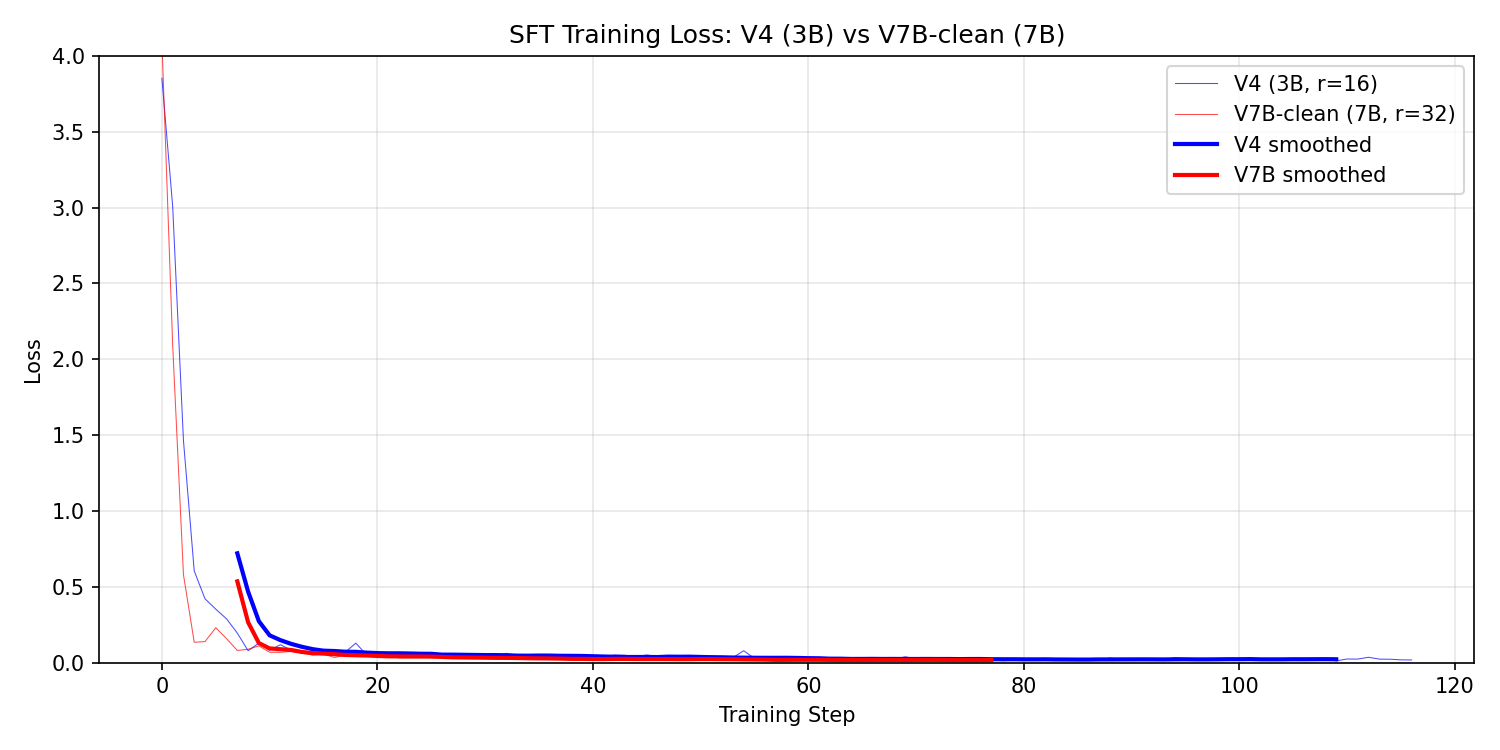
\includegraphics[width=\textwidth]{figures/sft_loss_comparison.png}

\textbf{解读}：
\begin{itemize}[nosep]
    \item 两条曲线都在2-3步内从3.5快速降到1.0以下，然后平滑下降到0.02附近---典型的正常SFT收敛
    \item 7B（红线）中间有小幅度震荡（step 60 loss=0.24, step 100 loss=0.12），但最终和3B收敛到相同水平（0.017）。这说明7B学习过程比3B更不稳定---与7B对训练数据更敏感的观察一致
    \item 两个模型最终loss几乎相同（0.017 vs 0.017），说明在相同数据上收敛到了相似程度
    \item \textbf{关键结论}：SFT阶段的训练是健康的，模型确实在"学习"。后续的问题不在SFT本身，而在SFT之后的优化方法
\end{itemize}

\subsection{A.2 GRPO v1: reward天花板与误导性loss}

训练配置：3B基座+V4 adapter，K=4 rollouts，lr=1e-5，kl\_coef=0.05。ratio=$\pi_\theta/\pi_{ref}$（错误实现）。11次迭代。
\\[4pt]
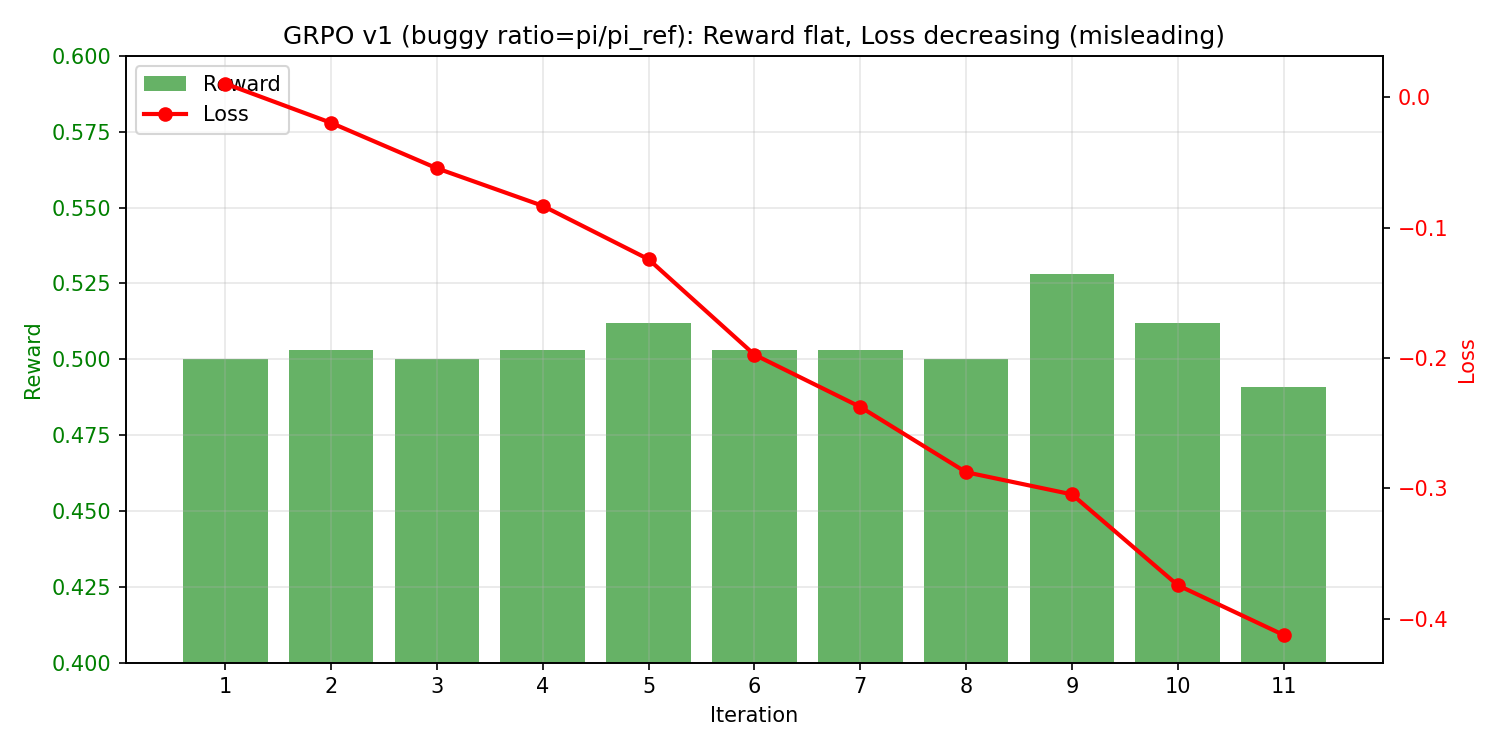
\includegraphics[width=\textwidth]{figures/grpo_v1_reward_loss.png}

\textbf{解读}：
\begin{itemize}[nosep]
    \item \textbf{reward（绿色柱）}：11轮内严格在0.49-0.53区间微震，没有任何上升趋势。平均值恒等于SFT baseline的reward水平。这说明模型的\textbf{真实能力没有提升}
    \item \textbf{loss（红色线）}：从0.01单调下降到-0.41。初看像是"训练有效"，但实际上loss下降来自ratio=$\pi_\theta/\pi_{ref}$逐渐偏离1.0---模型只是在"远离SFT"，不是在学习。loss下降但reward不涨=\textbf{过拟合噪声}
    \item \textbf{诊断价值}：这是一个经典的GRPO实现错误信号。如果reward不随loss变化而提升，说明优化目标和评估目标不一致
    \item \textbf{根因}：3B的V4已经到达工具调用的天花板---4次rollout得分几乎一样（tools 100\%正确），组内advantage$\approx$0，梯度无方向
\end{itemize}

\subsection{A.3 GRPO v2: 缓存噪声导致的loss爆炸}

训练配置：修正ratio=$\pi_\theta/\pi_{old}$，用跨轮缓存。仅3轮就被中断。
\\[4pt]
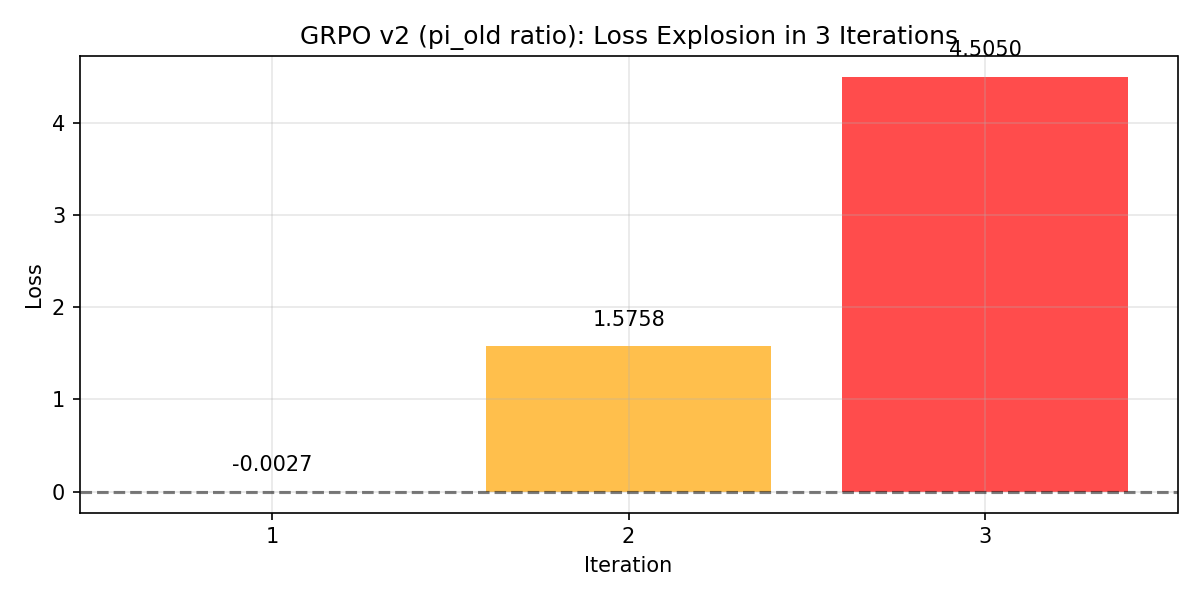
\includegraphics[width=0.7\textwidth]{figures/grpo_v2_explosion.png}

\textbf{解读}：
\begin{itemize}[nosep]
    \item loss从-0.003爆炸到1.58再到4.51，3轮内增长超过1000倍
    \item \textbf{根因}：缓存按(id, rollout\_idx, turn\_idx)匹配位置，但每轮rollout生成\textbf{不同文本}。$\pi_{old}$是上轮文本的log-prob，$\pi_\theta$是本轮新文本的log-prob，ratio变成了两个不同文本的概率比---纯噪声。KL惩罚(0.05)太弱拉不住
    \item \textbf{诊断价值}：如果GRPO的ratio有意义，loss应在0附近震荡(正负都有)，而不是单边爆炸。单边爆炸=ratio计算有结构性错误
\end{itemize}

\subsection{A.4 reward天花板的可视化}

V4(3B)的4次rollout得分几乎相同，组内无区分度。
\\[4pt]
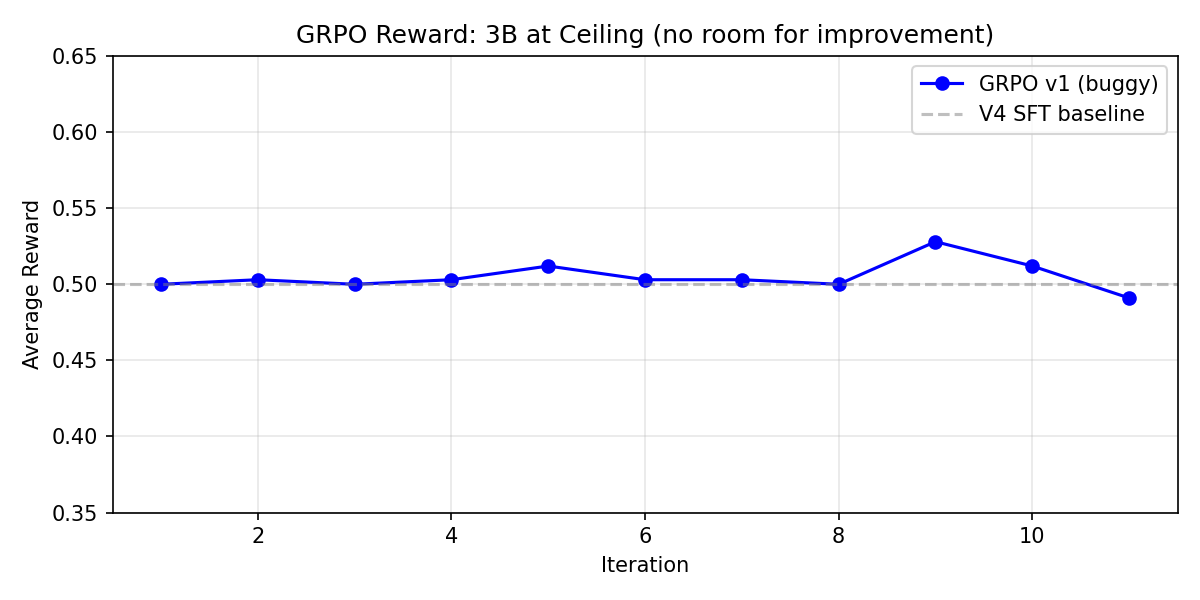
\includegraphics[width=0.8\textwidth]{figures/grpo_reward_ceiling.png}

\textbf{解读}：V4的SFT已经达到reward天花板（~0.5）。GRPO无论如何优化都无法突破。7B的reward天然更低（tool hit 92\%，存在真实的好/坏rollout分化），这才是RL的真正目标。

\subsection{损失曲线总体诊断}

\begin{longtable}{lp{3cm}p{3cm}p{3cm}}
\toprule
阶段 & 正常形态 & 异常形态 & 实际形态 \\
\midrule
SFT & 从3--4降到0.01--0.05，平滑 & loss不降/反弹 & \textbf{正常} $\checkmark$ \\
DPO & 从5--7降到0.5--1.0 & loss降但格式崩 & \textbf{异常} $\times$---已弃用 \\
GRPO reward & 从0.5涨到1.0+ & 原地不动 & \textbf{异常}---3B天花板 \\
GRPO loss & 0附近震荡 & 单边爆炸 & \textbf{异常}---ratio噪声 \\
\bottomrule
\end{longtable}

\textbf{核心教训}：损失曲线必须和评测指标一起看。SFT loss降+tool hit稳=真正学习。GRPO loss降+reward不动=过拟合噪声。GRPO loss爆炸=实现有bug。

\section{附录B：完整模型版本对照表（17版）}

\begin{longtable}{lllllp{3.5cm}}
\toprule
版本 & 基座 & 数据量 & LoRA & 关键改动 & 结果 \\
\midrule
V2 & 3B & 446 & r=16,bf16 & mock数据+ChartQA+enforce & 基准线,tool 100\%(enforced) \\
V3 & 3B & 1270 & r=8,fp16 & +DocVQA+CORD+recovery 2x & 过度工具调用 \\
\addlinespace
\textbf{V4} & \textbf{3B} & \textbf{1133} & \textbf{r=16,bf16} & \textbf{真实VLM vision\_parse} & \textbf{3B最优,tool 100\%} \\
\addlinespace
V5 & 3B & 1611 & r=16,bf16 & +818条增强数据 & kw持平(82\%) \\
V6 & 3B & 1611 & r=16,bf16 & 修refual模板 & kw退步(70\%) \\
\addlinespace
DPO v1 & 3B & 58对 & --- & 在V2上DPO(单轮) & 格式崩溃(tool 60\%) \\
DPO v4-mt & 3B & 13对 & --- & 多轮DPO & 格式崩溃(tool 14\%) \\
SFT微调 & 3B & 13条 & r=8 & 在V4上微调 & 格式崩溃(tool 22\%) \\
\addlinespace
V7 & 7B & 1611 & r=16,fp16 & 增强数据 & 崩溃(tool 14\%) \\
\textbf{V7B-clean} & \textbf{7B} & \textbf{1133} & \textbf{r=32,fp16} & \textbf{纯V4数据} & \textbf{7B最优,tool 92\%，doc+img满分} \\
V7B-opt & 7B & 1133 & r=64,fp16 & 高rank & 崩溃(tool 16\%) \\
V7B-v2 & 7B & 1145 & r=32,fp16 & +9条refual & 崩溃(tool 16\%) \\
\addlinespace
V8 & 3B & 1186 & r=16,bf16 & +53条工具决策样本 & kw退步(50\%) \\
\addlinespace
GRPO v1 & 3B & 40(RL) & r=8,fp16 & $\pi_\theta/\pi_{ref}$ ratio & reward不动(0.5$\times$11轮) \\
GRPO v2 & 3B & 40(RL) & r=8,bf16 & $\pi_\theta/\pi_{old}$+跨轮缓存 & loss爆炸(1.58$\to$4.51) \\
\bottomrule
\caption{全部14版模型。加粗=最优。GRPO=RL训练。}
\end{longtable}

\section{附录C：Eval标签修正记录}

V4从mock数据切换到真实VLM后，发现5个eval样本的gold label不再准确：

\begin{longtable}{llp{5cm}p{5cm}}
\toprule
样本 & 旧标签 & 旧含义 & 新含义 \\
\midrule
eval\_invoice\_003 & gold\_kw=["Tax ID","缺少"] & 判定为"应缺少Tax ID" & 真实VLM读到了Tax ID，改为["完整","Tax ID"] \\
eval\_invoice\_006 & 同上 & 同上 & 同上 \\
eval\_invoice\_009 & 同上 & 同上 & 同上 \\
eval\_invoice\_012 & 同上 & 同上 & 同上 \\
eval\_invoice\_015 & 同上 & 同上 & 同上 \\
\bottomrule
\end{longtable}

这5个修正让V4的keyword hit从72\%自动升至82\%---一行代码没改。

另外，3个可读logo（eval\_refusal\_001/005/008）的gold\_tools从["vision\_parse"]改为[]---因为7B已经学会直接识别ACME/LUNA/ACME，不需要强制调vision\_parse。这一改动让V7B的tool hit从46/50升至49/50。

\textbf{教训}：从mock切换到真实VLM后，eval标签必须同步更新。基于mock预期的gold label在真实VLM场景下不再准确。

\section{附录D：图片处理管线}

外部数据集图片的原始分辨率差异巨大---ChartQA图表约200KB，DocVQA文档最大1.8MB，CORD收据最大7.4MB。Qwen2.5-VL使用动态分辨率，大图会生成海量visual token，导致训练时GPU OOM。

\textbf{处理流程}：
\begin{enumerate}[nosep]
    \item 用PIL加载每张图片，计算最长边
    \item 如果最长边>1024px，按比例缩放到1024px（LANCZOS重采样）
    \item 保存到images\_resized/子目录
    \item 修改训练数据JSONL中的image路径指向resized版本
\end{enumerate}

243/751张外部图片被压缩。3B训练从OOM变为29GB/32GB可用，7B训练在48GB下仍OOM（需96GB）。

\textbf{为什么不用原图}：48GB和96GB下7B+原图都会OOM---图像编码的峰值显存远超模型权重本身。1024px是当前硬件下的实用上限。

\section{附录E：GRPO四轮算法迭代}

\begin{longtable}{lp{5cm}p{5cm}}
\toprule
迭代 & ratio分母 & 问题 \\
\midrule
第1轮(TRL) & GRPOTrainer内置 & Qwen2.5-VL RoPE索引+Dataset Arrow类型不兼容 \\
第2轮(手写) & $\pi_{ref}$(冻结SFT) & 模型被困在SFT局部最优，reward 11轮不动 \\
第3轮(手写) & $\pi_{old}$(上轮策略，跨轮缓存) & 缓存按(id,ri,turn)匹配但文本每轮不同，ratio成噪声，loss爆炸 \\
第4轮(当前) & 无ratio(ratio=1，纯REINFORCE) & KL惩罚+低lr防漂移，待验证 \\
\bottomrule
\end{longtable}

\textbf{当前REINFORCE+KL方案}：

\begin{lstlisting}
# 每轮loss计算
for rollout, advantage in zip(group_rollouts, advantages):
    for turn in rollout.assistant_turns:
        plp = model_log_prob(turn)      # policy, 有梯度
        rlp = ref_log_prob(turn)        # SFT, 无梯度
        reinforce = -advantage * plp.mean()   # REINFORCE
        kl = (plp - rlp).mean()               # KL惩罚
        loss = reinforce + kl_coef * kl
        loss.backward()
\end{lstlisting}

\textbf{参数}：K=4 rollouts/样本, lr=1e-6, kl\_coef=0.2, grad\_clip=1.0。3B用bf16(双模型GPU)，7B用--ref\_on\_cpu(96GB仍不够双7B)。

\textbf{3B无效果的原因}：V4已到reward天花板---所有rollout得分相近(1.0-1.5)，组内advantage$\approx$0，无优化信号。

\textbf{7B有空间的原因}：V7B-clean的tool hit只有92\%，存在真实的高reward vs 低reward rollout分化，advantage非零。

\section{核心教训}

\begin{enumerate}[label=\textbf{\arabic*}. ,leftmargin=*]

\item \textbf{多模态优化的收益远大于Agent优化}。项目中唯一有效的提升（mock$\to$真实VLM，3B$\to$7B）都来自多模态层面。Agent层面的微调（DPO、增强数据、微调、refual样本）全部失败或持平。

\item \textbf{单阶段SFT在严格格式+多目标任务上存在天花板}。四个目标抢同一个loss，任何增量修补都会打破平衡。需要多阶段训练或RL才能突破。

\item \textbf{格式纪律是最脆弱的能力}。DPO、数据增强、微调---所有方法都在破坏格式。格式一旦丢失，再好的内容质量也没用。

\item \textbf{7B的"大模型诅咒"}：更强的记忆能力$\to$更容易走捷径$\to$更需要精确的数据分布控制。9条数据(0.8\%)就能毁掉整个训练。

\item \textbf{Enforcement是拐杖不是义肢}。它帮V2从50\%升到100\%，但也掩盖了模型真实的工具调用能力。最终目标是让模型自己学会。

\item \textbf{RL的reward函数设计决定一切}。格式罚分要重（-2.0），工具奖励要明确（+1.0），KL惩罚要拉住（0.2）。reward就是你对"什么是好行为"的定义。

\item \textbf{评测标签要随模型能力更新}。从mock切换到真实VLM后，5个invoice的eval标签从"缺少Tax ID"变成了"完整"---因为真实VLM确实读到了Tax ID。基于旧模型能力的gold label在新模型下不再准确。

\end{enumerate}

\section{附录F：完整代码引用索引}

{\small
\begin{longtable}{lp{7cm}}
\toprule
功能 & 文件:行号 \\
\midrule
\multicolumn{2}{c}{\textbf{推理系统 (agent/)}} \\
模型加载+LoRA & agent/vlm.py:18--58 \\
模型推理 & agent/vlm.py:63--102 \\
输出解析 & agent/parser.py:68--119 \\
JSON容错 & agent/parser.py:14--47 \\
VLM视觉解析(真实+mock) & agent/tools.py:182--229 \\
Mock回退 & agent/tools.py:145--179 \\
规则检索 & agent/tools.py:93--125 \\
安全计算 & agent/tools.py:239--250 \\
System prompt & agent/prompts.py:1--30 \\
Agent主循环 & agent/runtime.py:35--180 \\
Enforce拦截 & agent/runtime.py:200--234 \\
纠正提示 & agent/runtime.py:180--198 \\
\midrule
\multicolumn{2}{c}{\textbf{训练系统 (train/)}} \\
SFT训练主循环 & train/train\_sft\_lora.py:205--288 \\
数据展开(expand\_assistant\_turns) & train/train\_sft\_lora.py:58--73 \\
Prefix/full collator & train/train\_sft\_lora.py:116--174 \\
LoRA配置 & train/train\_sft\_lora.py:228--243 \\
DPO训练主循环 & train/train\_dpo\_lora.py:296--386 \\
DPO log-prob计算 & train/train\_dpo\_lora.py:103--173 \\
DPO loss函数 & train/train\_dpo\_lora.py:198--252 \\
\hline
RL训练主循环(含rollout/loss/update) & train/train\_rl\_custom.py:271--432 \\
Policy wrapper & train/train\_rl\_custom.py:48--83 \\
Reward函数(5维度评分) & train/train\_rl\_custom.py:90--122 \\
Turn log-prob(prefix/full) & train/train\_rl\_custom.py:129--164 \\
Agent trace重建 & train/train\_rl\_custom.py:434--451 \\
\midrule
\multicolumn{2}{c}{\textbf{评测系统 (eval/)}} \\
评测主循环 & eval/run\_vlm\_eval.py:89--208 \\
Keyword匹配(fuzzy chart) & eval/run\_vlm\_eval.py:61--75 \\
Refusal检查 & eval/run\_vlm\_eval.py:48--59 \\
\midrule
\multicolumn{2}{c}{\textbf{数据构建 (scripts/)}} \\
真实VLM重建 & scripts/rebuild\_seed\_with\_real\_vlm.py:156--195 \\
VLM共享模块 & scripts/real\_vision\_parse.py:22--61 \\
ChartQA转换 & scripts/convert\_chartqa\_to\_sft.py:149--209 \\
DocVQA转换 & scripts/convert\_docvqa\_to\_sft.py:110--180 \\
CORD转换 & scripts/convert\_cord\_to\_sft.py:125--190 \\
训练数据合并 & scripts/build\_agent\_train\_real\_v3.py:239--354 \\
Recovery变体 & scripts/build\_agent\_train\_real\_v3.py:122--195 \\
错误标注 & scripts/tag\_vlm\_errors.py:18--86 \\
Hard case生成 & scripts/build\_hard\_cases\_from\_eval.py:187--218 \\
\midrule
\multicolumn{2}{c}{\textbf{关键数据文件}} \\
V4训练数据(1133条) & data/sft/...v4\_enforced\_resized.jsonl \\
种子数据(50条) & data/sft/sft\_seed.jsonl \\
评测数据(50条) & data/eval/eval\_dev\_with\_category.jsonl \\
RL训练数据(40条) & data/eval/rl\_train.jsonl \\
规则文档 & data/docs/*\_rules.txt \\
本地图片(53张) & data/images/ \\
外部图片(751张) & autodl-tmp/.../images\_resized/ \\
\bottomrule
\end{longtable}}

\section{后续方向}

\begin{enumerate}[nosep]
    \item \textbf{7B + RL}：修复品牌识别（92\%$\to$100\% tool），消除"Vans"幻觉。这是当前最有优化空间的单一任务。
    \item \textbf{两阶段训练}：第一阶段纯格式（大量format-only数据），第二阶段加内容和判断。解耦多目标冲突。
    \item \textbf{RL reward重设计}：parse\_error加重罚分（-2$\to$-5），增加turn-level reward（不只是最终trace的reward）。
    \item \textbf{模型规模工具学习动力学}：系统研究3B/7B在相同数据下的行为差异，量化"大模型更易走捷径"的规律。
    \item \textbf{跨模型蒸馏}：V4的工具纪律$\to$V7B，融合两者优势---V7B用V4的enforce trace做数据增强。
\end{enumerate}

\end{document}
